% 유형 023 41-07(인쇄 41쪽) — 정육면체의 전개도(십자 모양). 가운데 세로줄 1·2·9·8, 가운데 칸 2의 양옆에 3·7.
%   스캔 화질이 낮아 TikZ 로 다시 그림. 바깥 테두리는 실선, 접는 선은 원문대로 점선.
% 라벨은 원문에 있는 숫자만 넣는다(답은 그림에서 읽히지 않는다 — 전개도의 수는 문제의 주어진 조건).
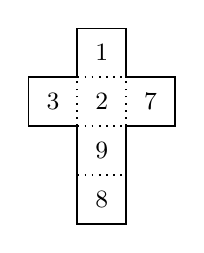
\begin{tikzpicture}[scale=0.62, line width=0.5pt]
  % 바깥 테두리
  \draw[line width=0.6pt] (1,4) -- (2,4) -- (2,3) -- (3,3) -- (3,2) -- (2,2) -- (2,0) -- (1,0) -- (1,2) -- (0,2) -- (0,3) -- (1,3) -- cycle;
  % 접는 선(원문의 점선)
  \draw[dotted, line width=0.6pt] (1,3) -- (2,3);
  \draw[dotted, line width=0.6pt] (1,2) -- (2,2);
  \draw[dotted, line width=0.6pt] (1,1) -- (2,1);
  \draw[dotted, line width=0.6pt] (1,2) -- (1,3);
  \draw[dotted, line width=0.6pt] (2,2) -- (2,3);
  \node[font=\small] at (1.5,3.5) {$1$};
  \node[font=\small] at (0.5,2.5) {$3$};
  \node[font=\small] at (1.5,2.5) {$2$};
  \node[font=\small] at (2.5,2.5) {$7$};
  \node[font=\small] at (1.5,1.5) {$9$};
  \node[font=\small] at (1.5,0.5) {$8$};
\end{tikzpicture}
